\documentclass[a4paper,11pt]{article}
\textheight 8.8in
\textwidth 6.0in
\parindent 0.3in
\topmargin -0.2in
\setlength{\oddsidemargin}{.25cm}
\usepackage{color}
\usepackage{graphicx}
\definecolor{light_grey}{gray}{0.7}
\usepackage[table]{xcolor}
\usepackage{subfig}
\usepackage{minted}
\title{LULC-Net: Generalized convolution neural network classfier for detecting land use changes from satellite data}
\date{}
\author{Rishu Saxena}

\begin{document}
\maketitle
Recently, convolution neural networks have been applied in wide
variety of complex, previously intractable, tasks such as image recognition
and semantic labeling and so on. 
This report presents preliminary findings on a novel application of CNN --
in understanding land use and land cover from images obtained from satellite data.
Land use change is described as changes in how humans use the surface
of the Earth (e.g., for agriculture, plantations, pastures, managed woods,
conservation, settlements, or leaving it alone as natural ecosystem).
Changes in land use lead to changes in albedo, the amount of sunlight reflected from 
the ground back into space (or, absorbed by the earth's surface), 
thereby directly affecting the temperatures of the surrounding area.
Significant and lasting changes in land use and land cover (LULC) have more
profound effects.
The past century has seen an exponential growth in human 
activities such as deforestation and urbanization causing significant changes
in land cover in several parts of the world \cite{Hansen}. Simultaneously,
significant changes in the global climate have also been observed, driven
in part by LULC change (LULCC) (e.g., \cite{FallEtAl}). LULCC also has impacts on a
wide variety of other ecosystem services. Monitoring LULCC across the globe,
therefore, has become the need {\it du jour}. Land use change detection
comprises any methodology used for determining the occurance and
nature of change in LULC.

We can observe land use and land cover through earth observation satellites (EOS) such as Landsat.
They capture images of the
Earth's surface at regular intervals using multiple spectral frequencies.
\begin{figure}
\centering
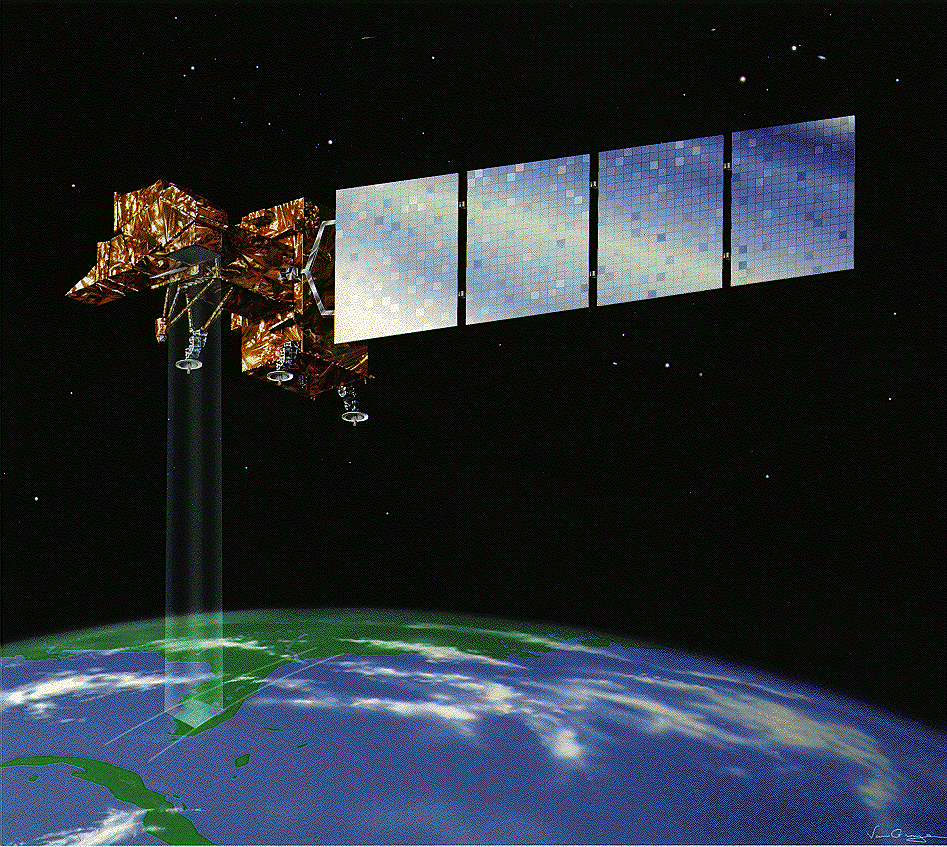
\includegraphics[width=3.00in, height=3.00in]{./landsat.png}
\caption{Earth observation satellites take images of the earth surface in patches at regular interval (Source: https://www.nasa.gov/).}
\end{figure}
These images hold valuable information that, if harnessed well, can be 
immensely helpful in understanding, monitoring, and managing our natural 
resources, as well as studying LULCC.
An excellent way of analyzing these satellite images for LULCC studies is
time series  analysis (or, temporal trajectory analysis). 
For time series analysis, several 
images of the scene under consideration, taken over a period of time, are
stacked together chronologically, and are subsequently analyzed (see figure~\cite{fig:stack}).
\begin{figure}
\centering
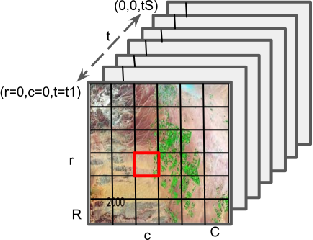
\includegraphics{./image_stack.png}
\caption{To detect land use change, satellite images are stacked chronologically.
The image stack yields a time series per pixel of the patch. All analysis are performed
on the time series.\label{fig:stack}}
\end{figure}
Commonly,
the time series for each pixel is treated individually; the full image
stack is thus a collection of many time series. The choice of spectral band(s)
varies from application to application. The objective is to
discover a `trend' in how different relevant variables (indicators) evolve over
time. Analysis is based on the behaviours of the time series of these
variables. In change detection analysis, when the trajectory of one or more of
the variables departs from the normal, a change is detected. 
Time series analysis for LULCC studies has been receiving increasing attention
in the last decade, specifically, after the Landsat data became freely
accessible in 2008 \cite{WoodcockLandsatFreeaccess}. Several time series analysis 
algorithms have been proposed by different groups in the remote sensing 
community.

\begin{figure}
    \centering
    \subfloat[before change]{{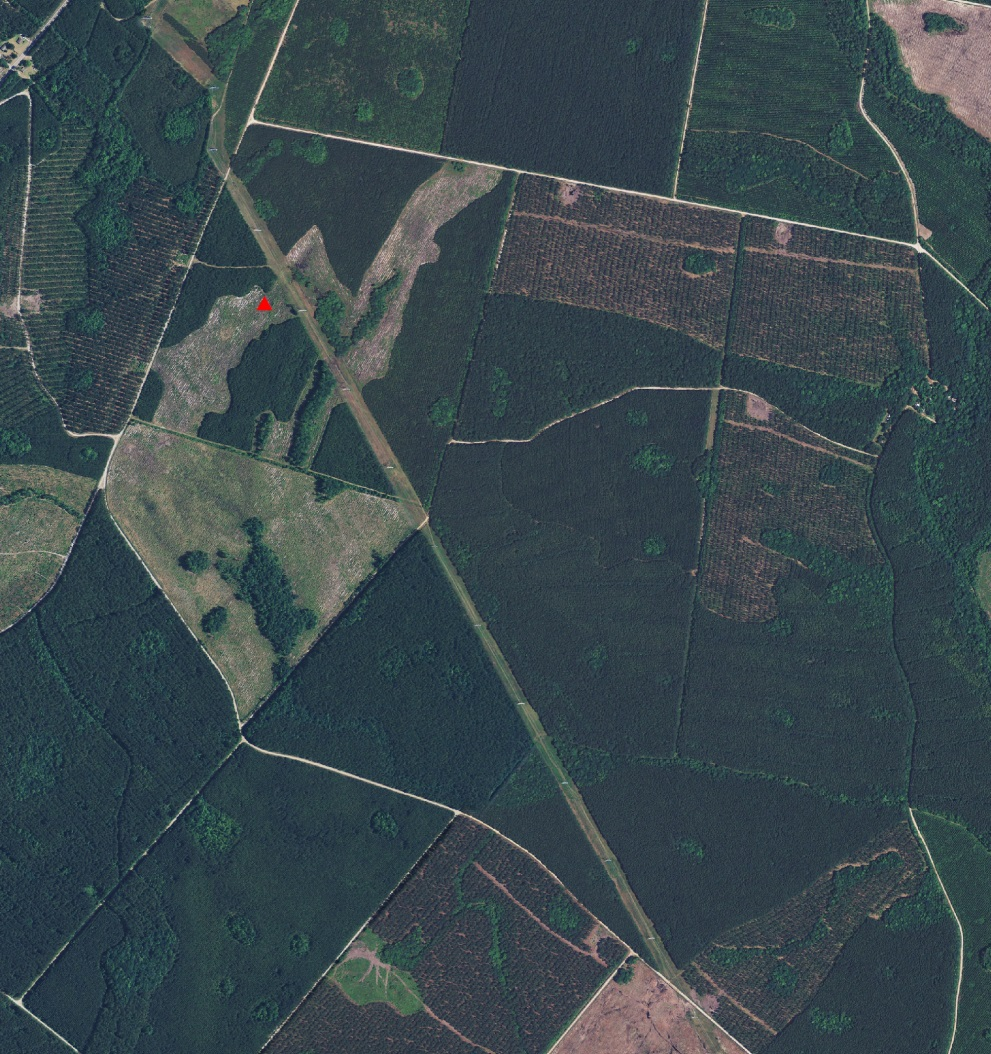
\includegraphics[width=5cm]{patch_pre_change.png} }}%
    \qquad
    \subfloat[after change]{{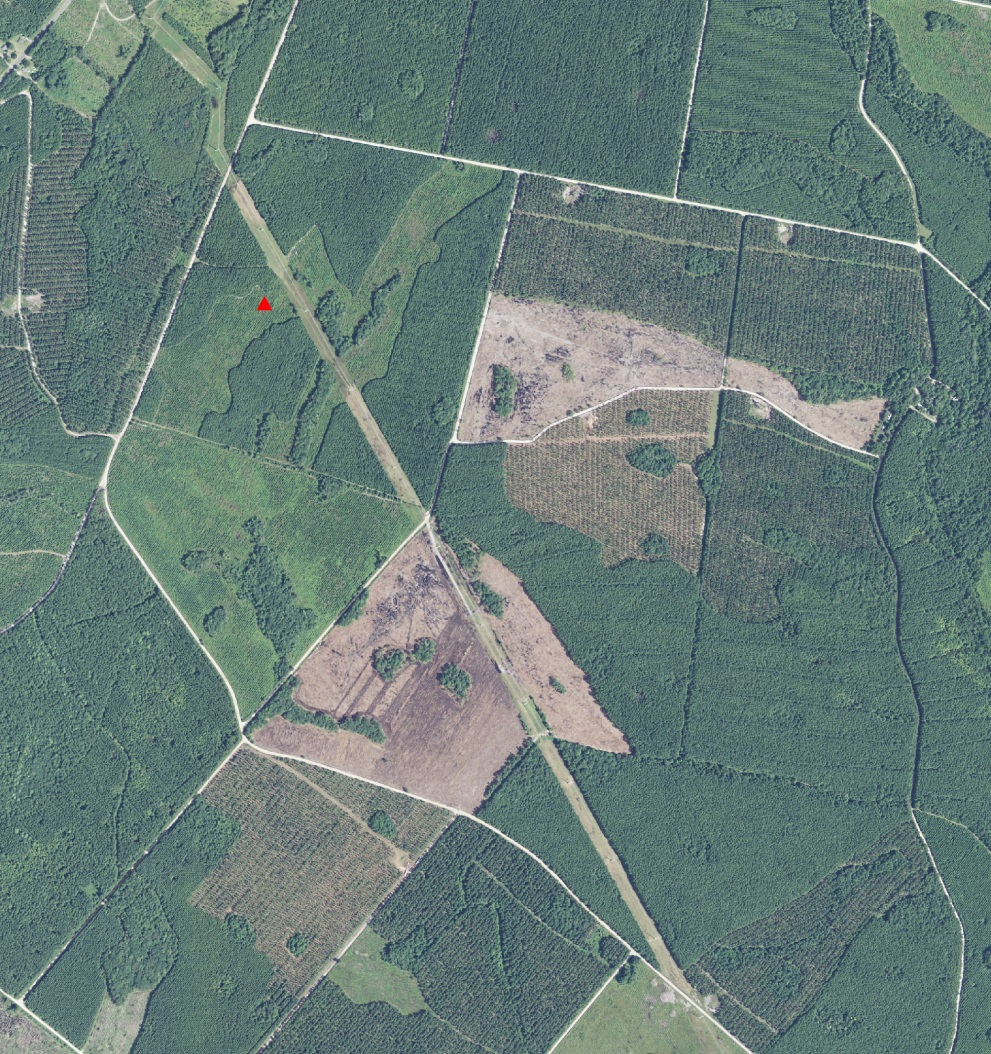
\includegraphics[width=5cm]{patch_post_change.png} }}%
    \caption{Image of patch pre and post change.}%
    \label{fig:example}%
\end{figure}
%%Add some example figures
%%add breakpoint
%%Due to lack of formal definition of breakpoints

Despite a plethora of time series analysis algorithms available in 
remote sensing, design and selection of algorithms for LULCC detection in remote
sensing appears to be almost always context specific. Most of the methods
proposed to date seem to perform well on the type of data that they are designed
for. Their performance on randomly picked datasets from across the
globe has not been studied. The onus of choosing an appropriate algorithm that
will perform well on their particular dataset falls on the user.
Unfortunately, no single algorithm designed so far seems to work for all
datasets \cite{lcmsCohen}. For example, the Western Antarctica as 
well as the Greenland Ice Sheets are beginning to collapse due to global warming, 
the melting leading to continually receding snow covers
at the respective locations. For these regions, using LULC algorithms based on
periodicity assumptions is expected to lead to incorrect predictions and/or false
alarms, although the nature and extent of this has not been studied yet.
Even if there were no global warming, mild shifts in the `phase' and `amplitude'
of seasons are known to take place \cite{petitjeanC}. Time warping techniques
\cite{petitjeanC} to deal with these issues may be helpful in some contexts, but
their accuracy and scalability has not yet been satisfactorily investigated.
Approaches based on periodicity and a moving window are possible, with 
additional computational costs.



This work proposes the use of a neural networks based approach for LULCC. 
One of the key hurdles in applying CNN approach for LULC is the lack of
quality annotated data LULC. Effective CNNs could be developed for
object recognition and semantic labeling because
vast amount of relatively high quality annotations of images could be harvested
from social media and the web in general.
Researchers from this data were able to build a  vast repository of semantically
annotated images which can then be used for training a CNN for various
complex image procesing tasks. Satellite image processing, though important, however, is a
niche scientific area with only a handful of scientist and engineers currently working on it.
In addition, image data from satellite  have various quality issues
such as relatively high level of noise, incorrect readings due to sensor malfuction,
influence of ambient enviorment and so on.
As such, obtaining breakpoint labels over the images in large quantity is a significant challenge.
The other primary difficulty in developing a universal algorithm for LULCC is that
that the input data cannot be modeled. Different datasets picked from across
the globe vary in trend, periodicity, mean and variance, etc., in addition to
real world aspects such as missing data and ambient noise (due to clouds,
sensor malfunction, pollution, and the like). Neural networks are based
on predictor-corrector approach. They do not make nor need any {\it a priori}
assumptions on the model, and instead, implicitly learn the model from the
training data itself, they have potential for being useful for a much wider
gamut of datasets. 
Other challenges include designing the neural netowrk approach, validation,
and scalability.

In this report, we investigate one approach to over this hurdle and build a CNN to detect land usage change
from satellite images.
In this work, we address the problem of building the training data,
and explore a canonical approach for classifying a time series as one
with change or a stable one. 
%%vocab: breakpoint labels
Our approach to derive breakpoint labels is based on polyalgorithm method for breakpoint detection
developed as part of my thesis.

The rest of this paper is organized as follows: Section 2 presents
background on state-of-the-art change detection algorithms available in 
remote sensing. Section 3 presents the proposed neural networks based
approach: training data generation, neural networks model, and the results.
Conclusions and future work are presented in Section 4.


\section{Generating Training data for CNN using Polyalgorithm and Timesync data}
%%What is polyalgorithm
The foundation for a polyalgorithm 
is laid using three distinct algorithms, viz., LandTrendR, EWMACD (Exponentially
Weighted Moving Average Change Detection), and BFAST (Breaks for Additive
and Seasonal Trends).
We briefly discuss the BFAST algorithm as it is one of the more effective techniques
for breakpoint detection.

{\bf Breaks For Additive and Seasonal Trend.} Amongst the state-of-the-art
LULCC detection algorithms in remote sensing, BFAST \cite{VerbesseltC} is found
to be most thorough and accurate in assessing change. This
is a recuresive residual based algorithm that considers every
single timepoint in the time series as a candidate breakpoint, computes the
least squares residuals for fits on either side of that timepoint, and
eventually selects the timepoints that yield lowest loeast squares residuals
as the breakpoints. Specifically, BFAST decomposes the given time series
iteratively into three components:
trend, seasonal, and noise. BFAST computes and evaluates least squares fits
in windows of increasing size. 
Qualitatively, (i) first the possibility of there being any structural change
in the given time series is determined by computing the partial sums of
residuals of least squares fits in windows (OLS-MOSUM). The limiting
process of these partial sums is the increments of a Brownian bridge 
process \cite{OLSMosum}. If the observations do have a structural change,
an ordinary linear least squares fit will result in large residuals
and, hence, in large partial sums. Therefore, the occurence of large values
in the process is an indication of the
presence of a structural change --- this probability being calculated 
from the Brownian bridge table.
(ii) If a structural change is indicated, a search for change 
location is done. {\it Each} interior time point $t$ is considered
a breakpoint (change location) candidate. 
A recursive residual is the error at time $t_j$ from the linear least squares
fit over the window $[t_i,\ldots, t_{j-1}]$. The breakpoints (change 
locations) are chosen so as to minimize the sum of squared 
recursive residuals over all windows
in between (omitting) the breakpoints.
This is done for both trend and seasonal components of the time series,
consecutively. A formal pseudocode for BFAST is presented in \cite{swwtHPC}.
\begin{figure}
\centering
    \subfloat[Harvest to Forest change]{{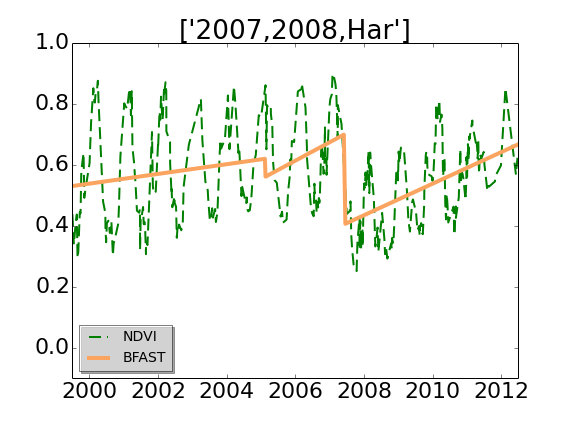
\includegraphics[width=5cm]{bfast_example1.png} }}%
    \qquad
    \subfloat[Fire in non-forest vegetation]{{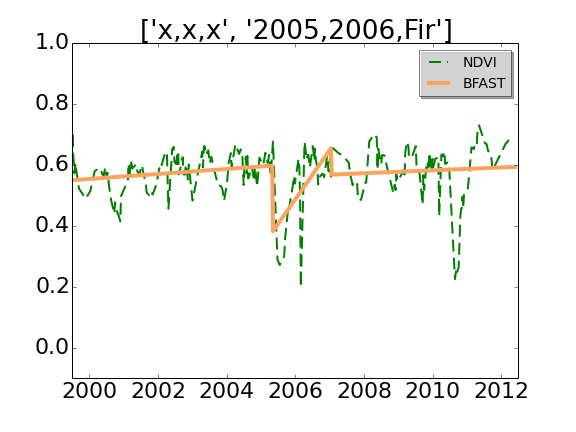
\includegraphics[width=5cm]{bfast_example2.png} }}%
    \caption{Figure illustrates result of BFAST algorithm on two patches that underwent land cover change.}%
    \label{fig:example}%
\end{figure}


{\bf Timesync data.} The state-of-the-art information on LULCC for a select
set of pixels is provided by the TimeSync dataset \cite{timeSync}.
This dataset is prepared using TimeSync Landsat time series 
visualization and change data collection tool \cite{timeSync}. This tool
enables disturbance characterizations for pixel-level samples of Landsat
time series data, relying on human interpretations of change as viewed
in image chip series, spectral index trajectories, high spatial resolution
image temporal snapshots from Google Earth, and other supporting products. 
Landsat image stacks spanning the years 1984 to 2014 and belonging to six
different path/rows (scenes) are considered for preparing TimeSync dataset.
From each scene, 300 pixels are chosen with random sampling, and without
regard to land cover. Thus there are 1800 pixels in all included in the 
dataset. For each of these pixels, the following attributes are noted:
occurence of disturbance, the first year of detection (a year between 1986
and 2011), the duration for gradual disturbances (in number of years), and
the causal agent class (harvest, fire, mechanical, decline, wind, other).
Of the 1800 pixels, 1303 pixels were forested at some point within the
26 year time period.
The work presented in this article utilizes the time series of the 
pixels included in TimeSync data and the corresponding disturbance 
occurence information.
The results presented are limited to the time period 2000--2012.
Despite the tedious, conscentious efforts that TimeSync dataset has
been prepared with, disagreement is sometimes found between the NDVI 
trajectory of a pixel and the Timesync change information. 

\section{LULC-Net: A neural network for land use change detection}
We utilize a generic convolutional neural network (CNN)
for our problem. Our network consists of five layers --- first three 
convolutional, and next two fully connected. 

For the convolutional layers, $32$ filters each are used for the first
two layers, $64$ for the third layer. The convolution kernel has a
receptive field of size $3\times 3$. A stride of one pixel is used.
`ReLu' (Rectified Linear Units) is used as the activation function. ReLu
is defined as $$ f(x) = \max(0, x),$$
where $x$ is the input to the neuron. Networks that train with ReLu activation
allow efficient gradient propagation (no vanishing or exploding gradients)
and efficient computation (only comparison, addition, and 
multiplication). ReLu based networks are several times faster than networks
with other commonly used activation functions.
Each activation is followed by a max-pooling layer. Overlapping
pooling is used, with neighborhoods of size $2\times 2$,
and the centers of the neighborhoods $1$ pixels apart. 

The (pooled) output of the third layer is flattened out, and 

Dropout is a technique used to prevent overfitting and co-adaptations
of neurons by setting the output of any neuron to zero with probability
$p$.

Keep a moving average of the squared gradient for each weight

Data augmentation and Dropout are used to reduce overfitting.

Figure 1 diplays the NDVI trajectories of two pixels.

\begin{table}
\centering
\caption{Runtime Configuration}
 \rowcolors{2}{gray!25}{white}
  \begin{tabular}{cc}
  software & version \\
  GCC & 5.2 \\
  CUDA & 8.0.61 \\
  ATLAS & 3.0.12 \\
  Python & 2.7.13 \\
  PyCuda & 2016.1.2 \\
  Theano & 0.8.2 \\
  libgpuarray &  3.0 \\
  PyGPU & 0.7.5 \\
  \end{tabular}
\end{table}

\subsection{Implementation in Keras}
\paragraph{Header}
\begin{minted}{python}
import matplotlib
matplotlib.use("Agg")
import matplotlib.pyplot as plt
from keras.preprocessing.image import ImageDataGenerator
from keras.models import Sequential
from keras.layers import Conv2D, MaxPooling2D
from keras.layers import Activation, Dropout, Flatten, Dense
from keras import backend as K
import numpy as np
\end{minted}

\paragraph{Initialization}
\begin{minted}{python}
img_width, img_height = 204, 153
train_data_dir = 'rs_data/train/'  
validation_data_dir = 'rs_data/validation' 
test_data_dir = 'rs_data/test'
nb_train_samples = 100  
nb_validation_samples = 50  
epochs = 3 
batch_size =1
K.set_image_data_format('channels_first')
input_shape = (3, img_width, img_height)
\end{minted}

\paragraph{The Model}
\begin{minted}{python}
model = Sequential()
model.add(Conv2D(32, (3, 3), input_shape=input_shape))
convout_l1_act = Activation('relu') 
model.add(convout_l1_act)
convout_l1_mp = MaxPooling2D()  #(pool_size=(2, 2))
model.add(convout_l1_mp)


model.add(Conv2D(32, (3, 3)))
convout_l2_act = Activation('relu')
model.add(convout_l2_act)
convout_l2_mp = MaxPooling2D()
model.add(convout_l2_mp)  #MaxPooling2D(pool_size=(2, 2)))

model.add(Conv2D(64, (3, 3)))
convout_l3_act = Activation('relu')
model.add(convout_l3_act)
convout_l3_mp = MaxPooling2D()  #pool_size=(2,2)
model.add(convout_l3_mp)

model.add(Flatten())
model.add(Dense(64))
model.add(Activation('relu'))
model.add(Dropout(0.5))
model.add(Dense(1))
model.add(Activation('sigmoid'))

model.compile(loss='binary_crossentropy',
              optimizer='rmsprop', metrics=['accuracy'])
model.summary()
\end{minted}

\paragraph{Training and Validation}
\begin{minted}{python}
train_datagen = ImageDataGenerator(rescale=1./255, \
                                   shear_range=0.2,zoom_range=0.2, horizontal_flip=False)
test_datagen = ImageDataGenerator(rescale=1. / 255)
train_generator = train_datagen.flow_from_directory(train_data_dir,
    target_size=(img_width, img_height),
    batch_size=batch_size, shuffle=False, class_mode='binary')

validation_generator = test_datagen.flow_from_directory(validation_data_dir,
    target_size=(img_width, img_height), batch_size=batch_size, class_mode='binary')

model.fit_generator(train_generator,
    steps_per_epoch=nb_train_samples // batch_size,
    epochs=epochs, validation_data=validation_generator,
    validation_steps=nb_validation_samples // batch_size)
    
\end{minted}

\paragraph{Testing}
\begin{minted}{python}
test_generator = test_datagen.flow_from_directory(
         test_data_dir,
         target_size=(img_width, img_height),
         batch_size=batch_size,
         class_mode=None,  # only data, no labels
         shuffle=False)  # keep data in same order as labels

probabilities = model.predict_generator(test_generator, 500)
#print probabilities

from sklearn.metrics import confusion_matrix
import numpy as np
from sklearn.metrics import classification_report

y_true = np.array([0] * 70 + [1] * 70)
y_pred = probabilities > 0.5
print(classification_report(y_true, y_pred))
tn, fp, fn, tp = confusion_matrix(y_true, y_pred).ravel()

print tn, fp
print fn, tp

\end{minted}

\subsection{Visual interpretation of the generated model}
\begin{figure}
\centering
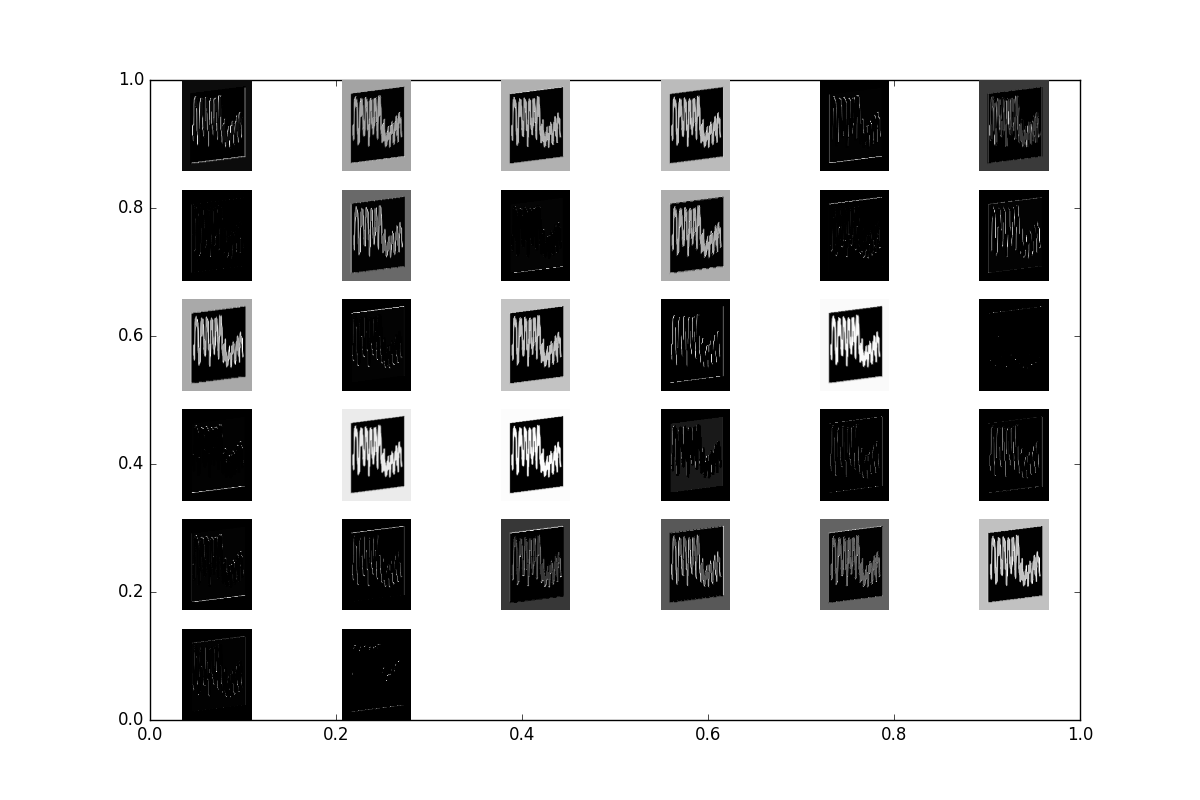
\includegraphics[width=5.00in]{layer1_act.png}
\end{figure}

\begin{figure}
\centering
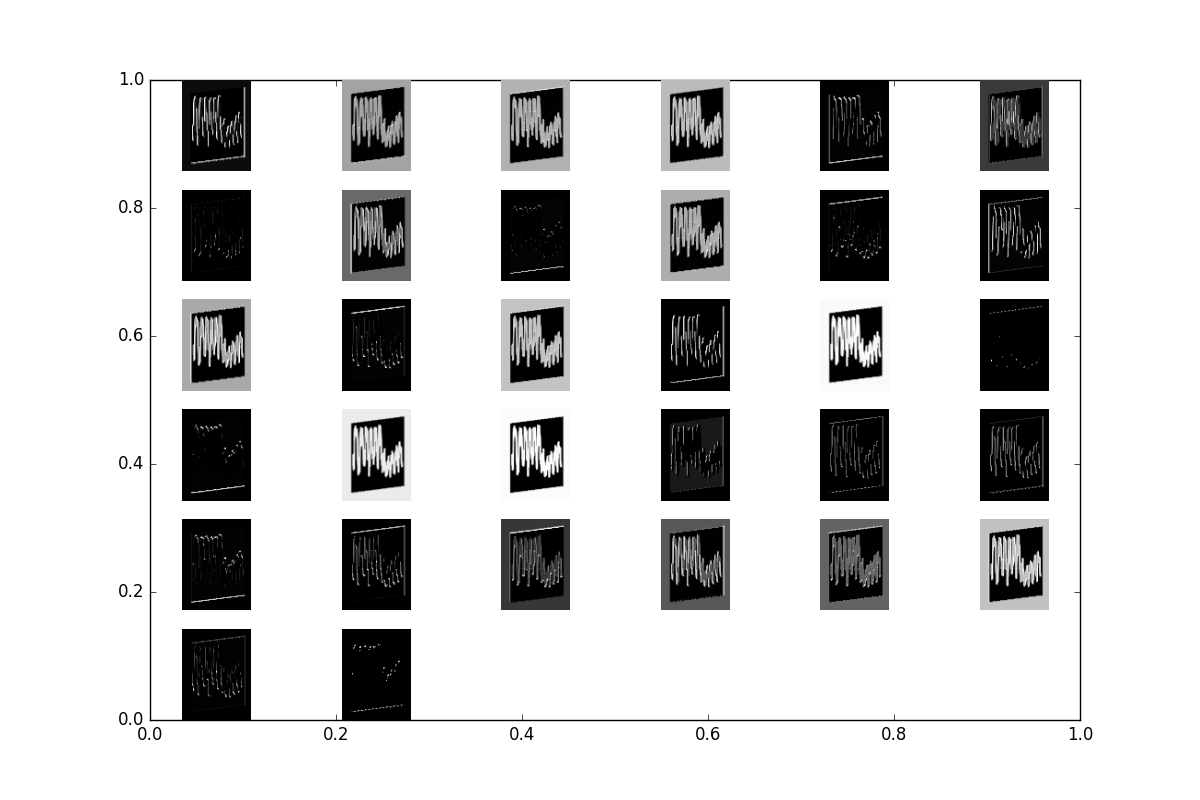
\includegraphics[width=5.00in]{layer1_mp.png}
\end{figure}


\begin{figure}
\centering
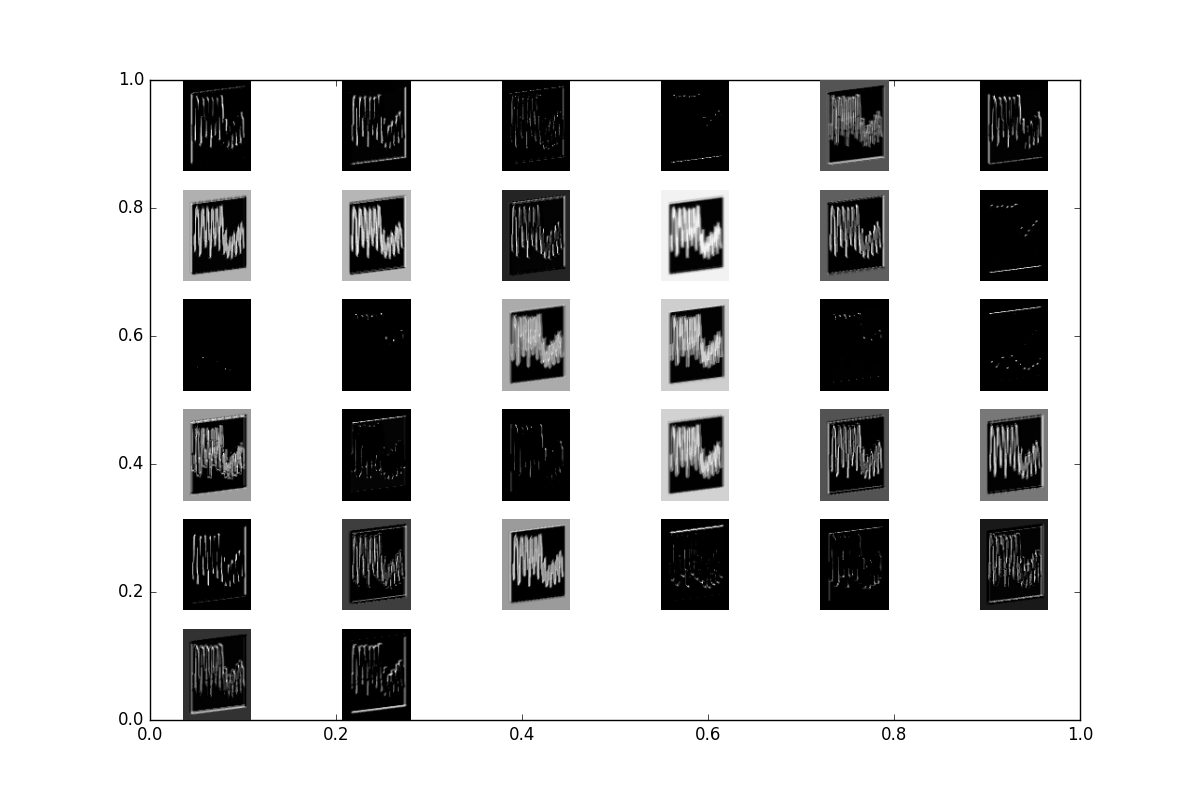
\includegraphics[width=5.00in]{layer2_act.png}
\end{figure}

\begin{figure}
\centering
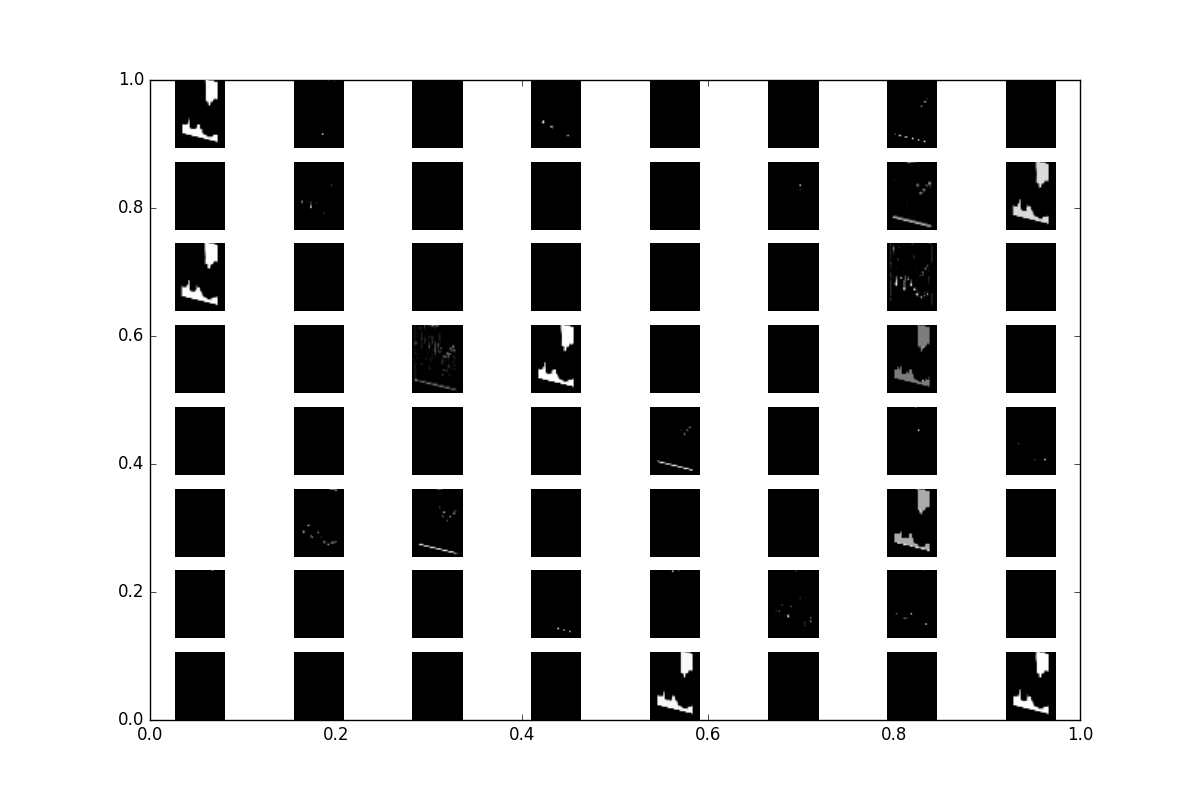
\includegraphics[width=5.00in]{layer3_act.png}
\end{figure}

\begin{figure}
\centering
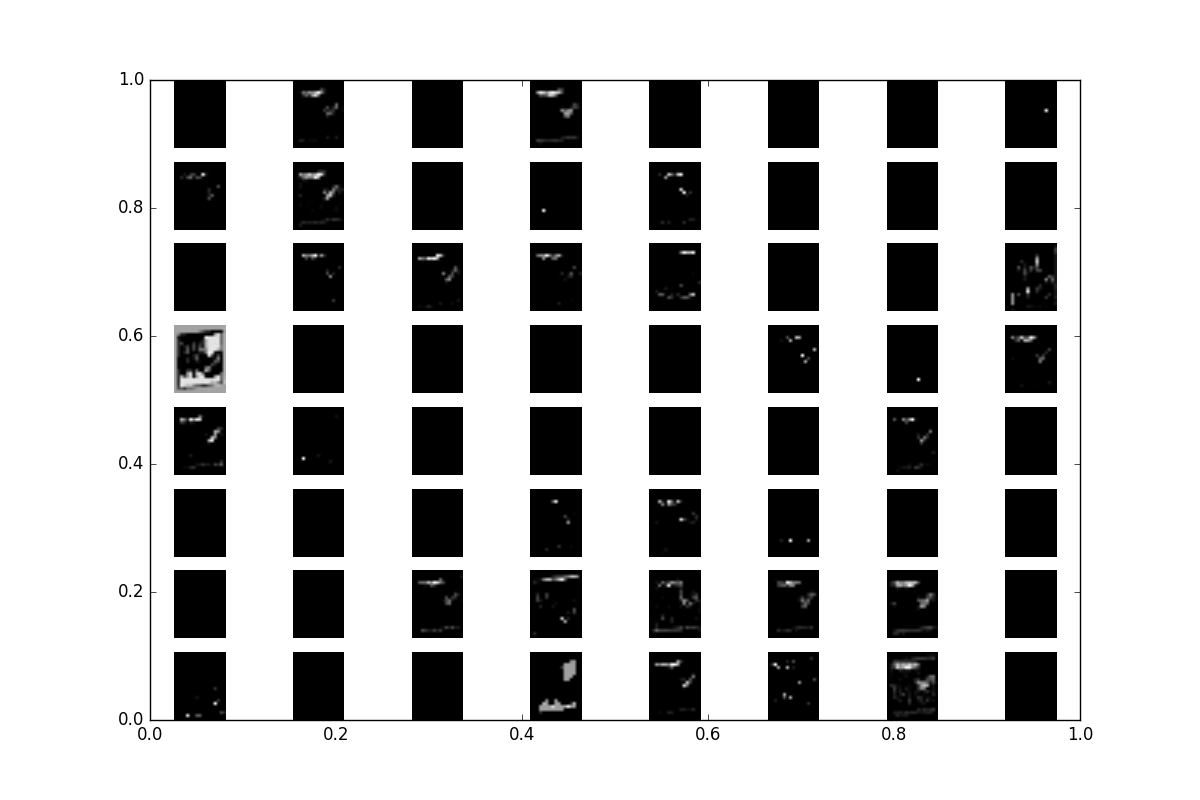
\includegraphics[width=5.00in]{layer3_mp.png}
\end{figure}



%% \begin{figure}[!ht]
%% \begin{centering}
%% \includegraphics[width=0.45\textwidth]{/home/rishu/research/thesis/presentations/thesis/rs_data/train/change/23038037.png}
%% \includegraphics[width=0.45\textwidth]{/home/rishu/research/thesis/presentations/thesis/rs_data/train/change/24038009.png} 
%% \end{centering}
%% \end{figure}

%{ \midinsert
%{ \centerline{\epsfxsize=14truepc\epsffile{24038009.eps}}
%{ \vskip -5pt
%{ \centerline{(a) Change.}
%{ \centerline{\epsfxsize=14truepc\epsffile{23038037.eps}}
%{ \vskip -5pt
%{ \centerline{(b) Stable.}
%{ \centerline{\caption{1}{Example trajectories.}}
%{ \endinsert




%%About timesync
\end{document}
